\documentclass[]{article}

\usepackage{ngerman}
\usepackage{comment}
\usepackage[ngerman]{babel}
\usepackage[utf8]{inputenc}
\usepackage[T1]{fontenc}
\usepackage{amsmath}
\usepackage{graphicx}
\usepackage{float}


% Title Page
\title{3D Vision LU}
\author{Christian Br\"andle \\
\texttt{Matr.Nr.: 1428543}
\and Stefan Zaufl \\
\texttt{ Matr.Nr.: 0925357}
\and Dominik Sch\"orkhuber\\
\texttt{ Matr.Nr.: 1027470}}

\begin{document}

\maketitle

%\begin{abstract}
%\end{abstract}

\section{Einleitung}  % dominik
In dieser Übung wurden von uns selbst gewählte Objekte mit einem 3D-Laserscanner virtualisiert. Dieses Dokument enthält alle Schritte des Scan- und Bearbeitungsvorganges. Eine abschließende Evaluation und ein Vergleich mit Autodesk 123D Catch zeigt die Qualität und Genauigkeit der erzeugten Modelle. 

\section{Modelle}
\subsection{}
\subsection{}
\subsection{Sparschwein}
\begin{figure}[!h]
\caption{Sparschwein}
\centering
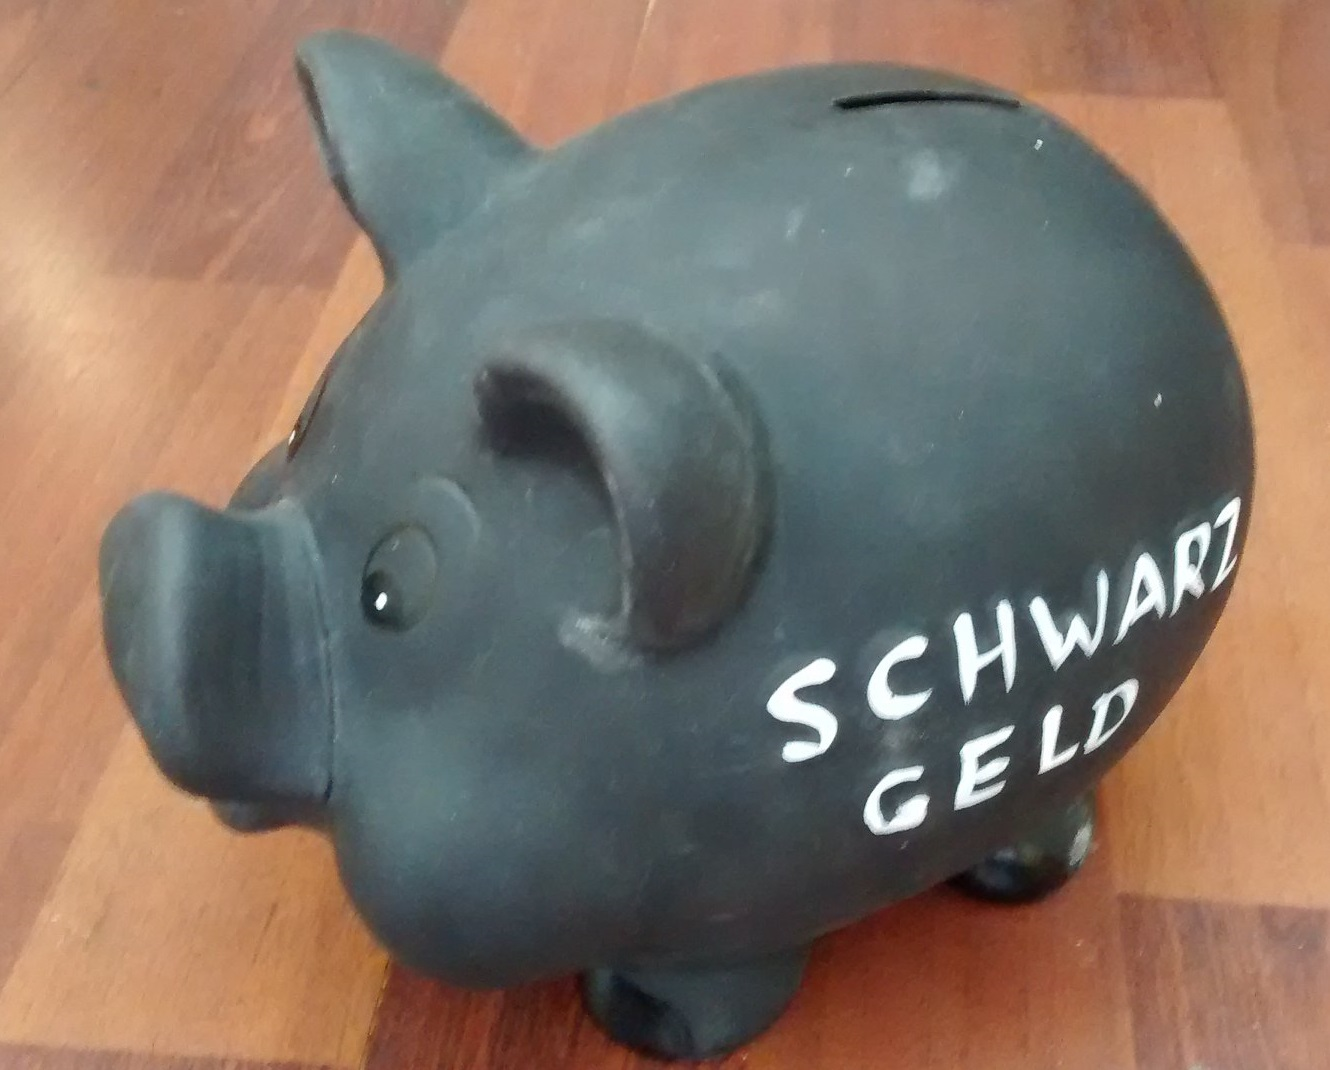
\includegraphics[scale=0.25]{images/sparschwein/photo.jpg}
\end{figure}

\section{3D Scanning} % stefan

Die Scandaten wurden $25$ Körperscans und $15$ Scans des Kopfes vorgenommen.
Die Scans des Kopfes wurden mit einer anderen Linse vorgenommen um eine erhöhte Auflösung im Speziellen des Gesichtes zu erreichen.

% Probleme
\subsection{}
\subsection{}
\subsection{Sparschwein}
Das Sparschwein Modell ist geometrisch nicht komplex, dennoch stellt es für den Minolta 3D-Scanner eine Herausforderung dar. Da das Modell sehr dunkel ist wird  nur ein sehr kleiner Anteil des Laser Lichts reflektiert. Um das zu kompensieren wurde beim Scanvorgang die Intensität des Lasers manuell erhöht. Weiters besitzt das Objekt einige sehr stark reflektierende Teile welche durch den Scanner schlecht bis gar nicht erfasst werden. In den Scans erscheinen diese Bereiche als Löcher. An den reflektierenden Bereichen konnte keine Oberfläche rekonstruiert werden. Glücklicherweise sind diese Bereiche nicht sehr groß und können in der Nachbearbeitung automatisch geschlossen werden.

\section{Nachbearbeitung in Geomagic} % christian

1. Globale Registrierung in Gruppen
2. Manuelle Registrierung der Gruppen, n-punkt
3. Vereinigen der registrierten Meshes

4. Nachbearbeitung
- Glätten, Spitzen entfernen, Mesh Doctor, löcher füllen
bis modell wasserdicht
5. sandpapier für feine nachbearbeitung


Zunächst wurden alle $40$ Scans gruppiert und manuell in den Gruppen zueinander registriert, da eine automatische Registrierung in den meisten Fällen fehlschlug.

Danach wurden die einzelnen Gruppen zueinander registriert um eine Gesamtdatenbasis des Modells zu erhalten.

Im Anschluss wurden auf den einzelnen Scans Fehler an den Scanrändern und bzw. überflüssige Teile der Scans von der Scanplatte entfernt.

Eine erneute Registrierung der bereinigten Daten verbesserte die Passgenauigkeit etwas. 

Das merging wurde auf Basis von allen Scans und auf Basis einer reduzierten Anzahl von Scans vorgenommen um Überlagerungen von identischen Scandaten zu vermeiden.

Im der Reduktion wurde auf die detailierten Facescans und auf die doppelt vorhandenen 360 Grad Scans der aufrechten Figur zugunsten eines besseren Rausch- bzw. Interpolationsverhaltens verzichtet.

\subsection{Waterproof 3D Model}

Das Schließen des Modells erforderte manuelle Arbeit für jedes einzelne Loch. Das beste Vorgehen bestand darin, die Umgebung des Loches von von allen störenden Artefakten zu befreien welche die 2D Mannigfaltigkeit des Meshes in diesem Bereich stören. Danach wird das Loch unter Berücksichtigung der Krümmung der umgebenden Oberfläche geschlossen.

% Nachbearbeitung und Probleme
\subsection{}
\subsection{}
\subsection{Sparschwein}
Durch die einfache Geometrie des Modells war auch die Nachbearbeitung der Oberfläche relativ einfach. Fast alle Bereiche der Oberfläche weisen eine sehr niedrige Krümmung auf. Dadurch hatte das rekonstruierte Modell auch schon vor der Nachbearbeitung nur sehr wenige Fehler. Am meisten Probleme bereitete der Münzeinwurfschlitz. Da die Hülle des Sparschweins nur wenige Millimeter dick ist wurde innerhalb des Schlitzes keine Geometrie aufgenommen. Ein automatisches Schließen des Bereiches hat erst nach einigen Versuchen zum gewünschten Ergebnis geführt, da je nach dem wie viel Geometrie gelöscht wurde sich auch die automatische Rekonstruktion verändert. 

\section{Evaluierung}
Um die Qualität der 3D-Scans zu beurteilen wurden Messungen an den realen Objekten durchgeführt und mit Messungen an den erzeugten Modellen verglichen.

% Messungen
\subsection{}
\subsection{}
\subsection{Sparschwein}
Für das Sparschwein wurden 7 Messungen durchgeführt und eine Genauigkeit von $\pm 1$mm festgestellt.
% wenns bei euch auch gleich ist vll in einem absatz alle beschreiebn

\section{Structure from Motion mit 123d Catch} % dominik

Autodesk 123d Catch ist eine Online Platform für Structure from Motion rekonstruktion. Zunächst werden Bilder des Objektes in konzentrischen Kreisen und aus mehreren Winkeln aufgenommen. Dabei ist es wichtig für eine gleichbleibende Beleuchtung zu sorgen. Am besten verwendet man mehrere Lampen die das Objekt gleichmäßig ausleuchten. Beim Aufnehmen der Bilder muss man sehr darauf achten keine Schatten auf das Objekt zu werfen. Nachdem man ~40+ Bilder aufgenommmen hat werden diese mit der 123d Catch Applikation hochgeladen und automatisch verarbeitet. Sobald der Vorgang abgeschlossen ist kann man das fertige Modell herunterladen. Die Rekonstruktion nimmt mit einer Berechnungszeit von ca. 45 Minuten sehr viel Zeit in Anspruch da die gesamte Verarbeitung der Daten am Server passiert. Ein großer Vorteil der Technologie ist dass keine spezielle Hardware benötigt wird. Sogar eine Handykamera reicht bereits aus um gute Ergebnisse zu erzielen.

% Vergleich der einzelnen Modelle
\subsection{}
\subsection{}
\subsection{Sparschwein}
Im Gegensatz zum Laserscanner hat 123d Catch große Probleme das Sparschwein zu rekonstruieren. Die Structure from Motion Technik verwendet Bildfeatures um die Bilder zueinander zu registrieren. Leider hat das Modell aber nur sehr wenige verwendbare Features. Entsprechend schlecht fällt das Ergebnis aus. In einem ersten Versuch wurden die Bilder so aufgenommen dass das Sparschwein das ganze Bild ausfüllt. In diesem Fall konnte 123d Catch überhaupt keine Registrierung erreichen. Um die Bilder mit Features anzureichern wurden die Aufnahmen in weiteren Versuchen aus etwas größerer Entfernung aufgenommen. Die Oberfläche konnte dann erfolgreich Rekonstruiert werden, wenn auch nur in sehr niedriger Qualität. In Bereichen wo Features vorhanden sind ist die Rekonstruktion durchaus detailliert. Man beachte den Schriftzug an der rechten Seite.

\begin{figure}[!h]
\caption{Vergleich mit 123d catch}
\centering
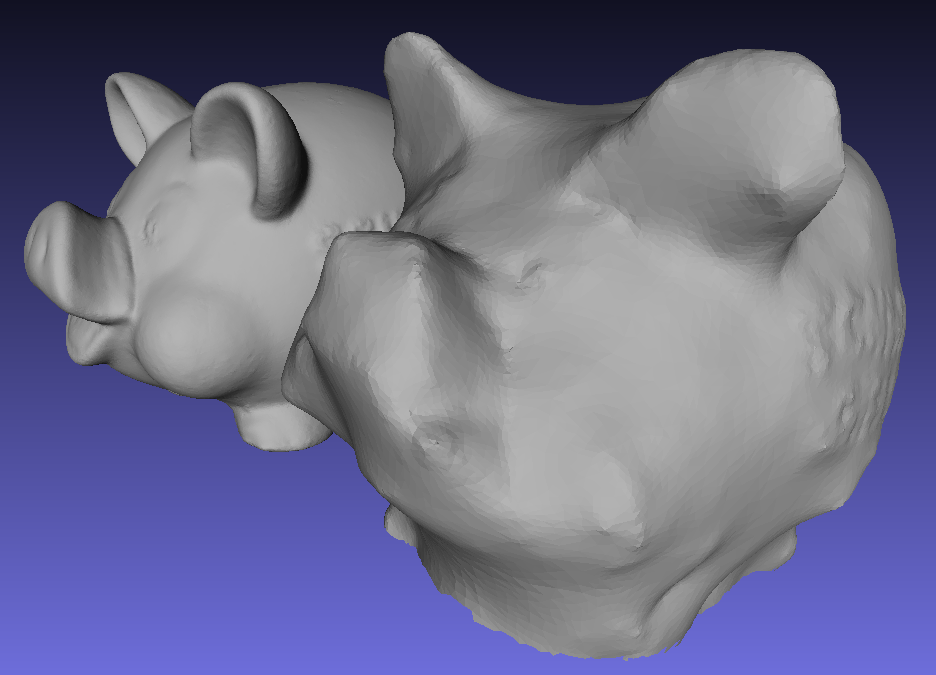
\includegraphics[width=80mm]{images/sparschwein/123d_Vergleich} % ersetzen
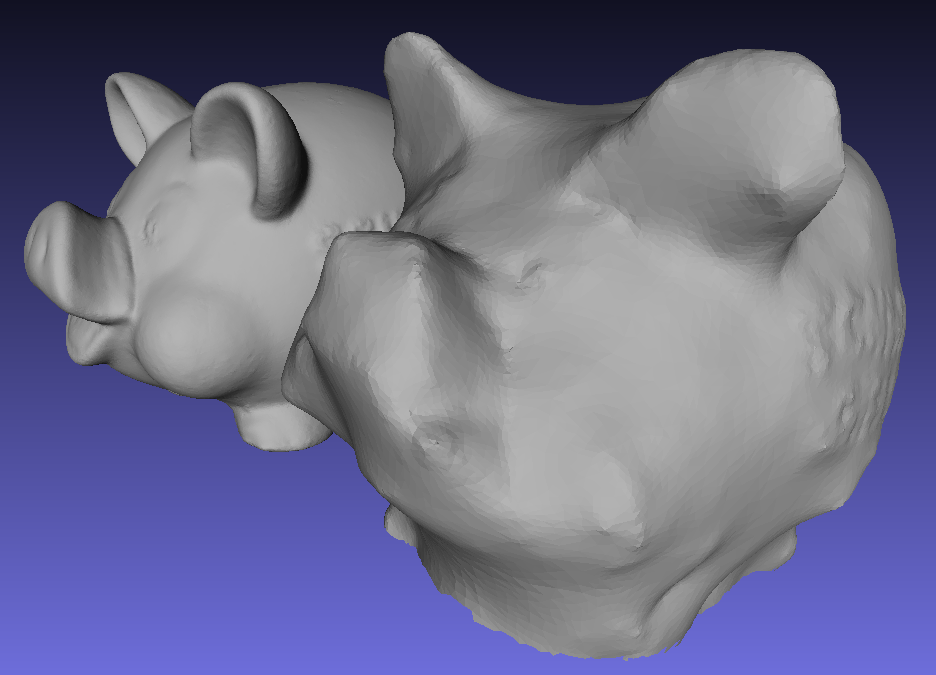
\includegraphics[width=80mm]{images/sparschwein/123d_Vergleich} % ersetzen
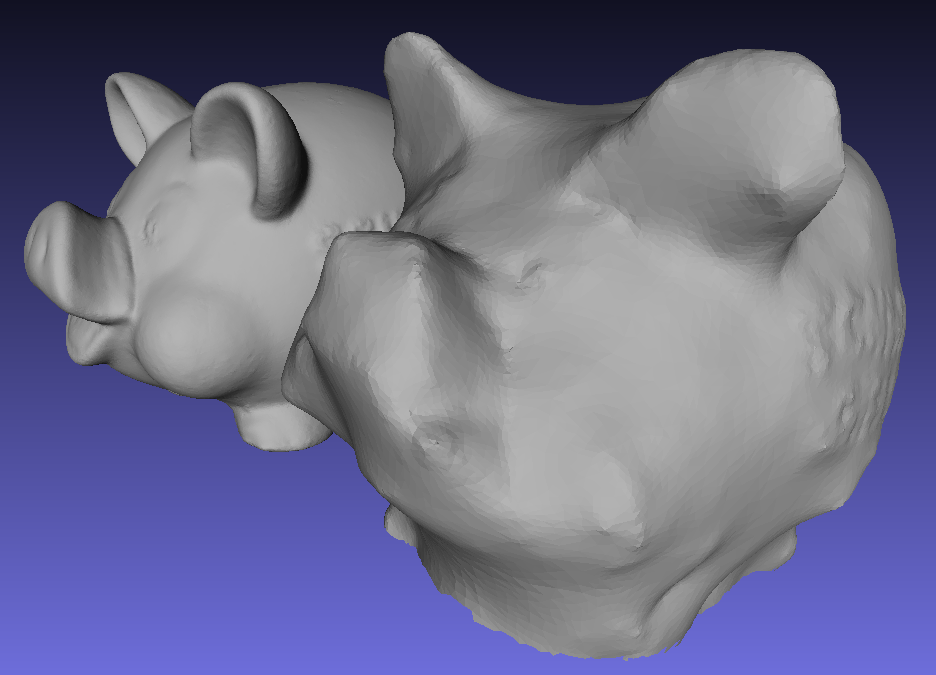
\includegraphics[width=80mm]{images/sparschwein/123d_Vergleich}
\end{figure}

\begin{figure}[!h]
\centering
\caption{Finale Modelle}
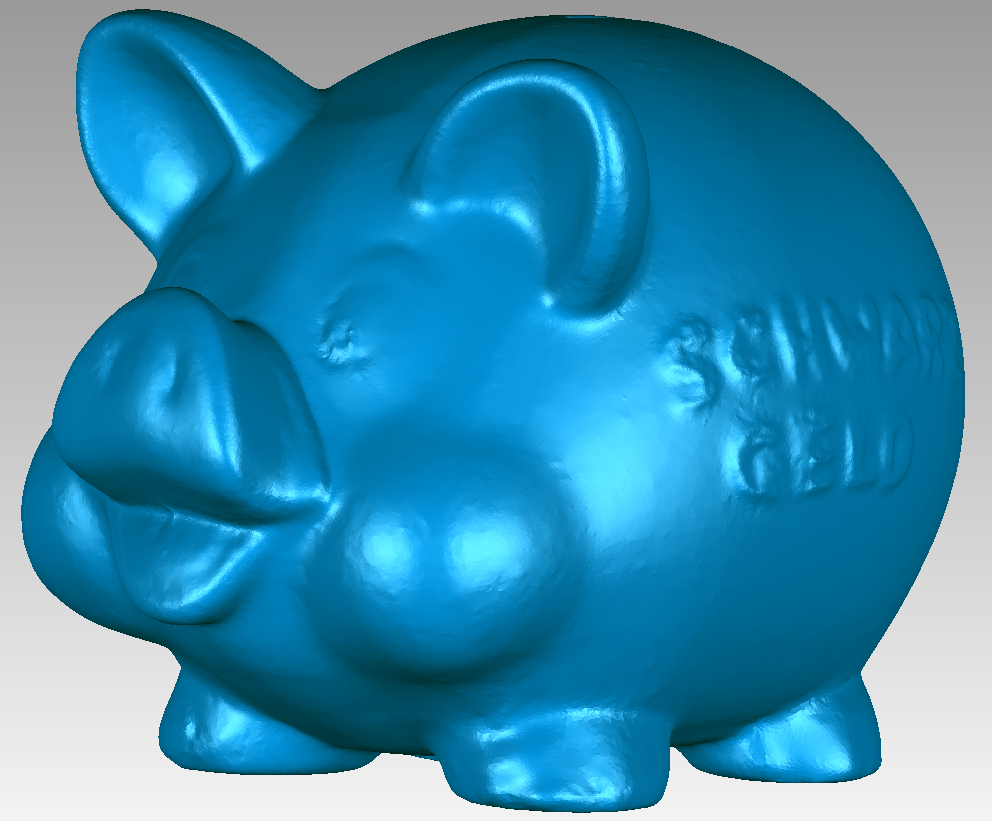
\includegraphics[width=80mm]{images/sparschwein/final} % ersetzen
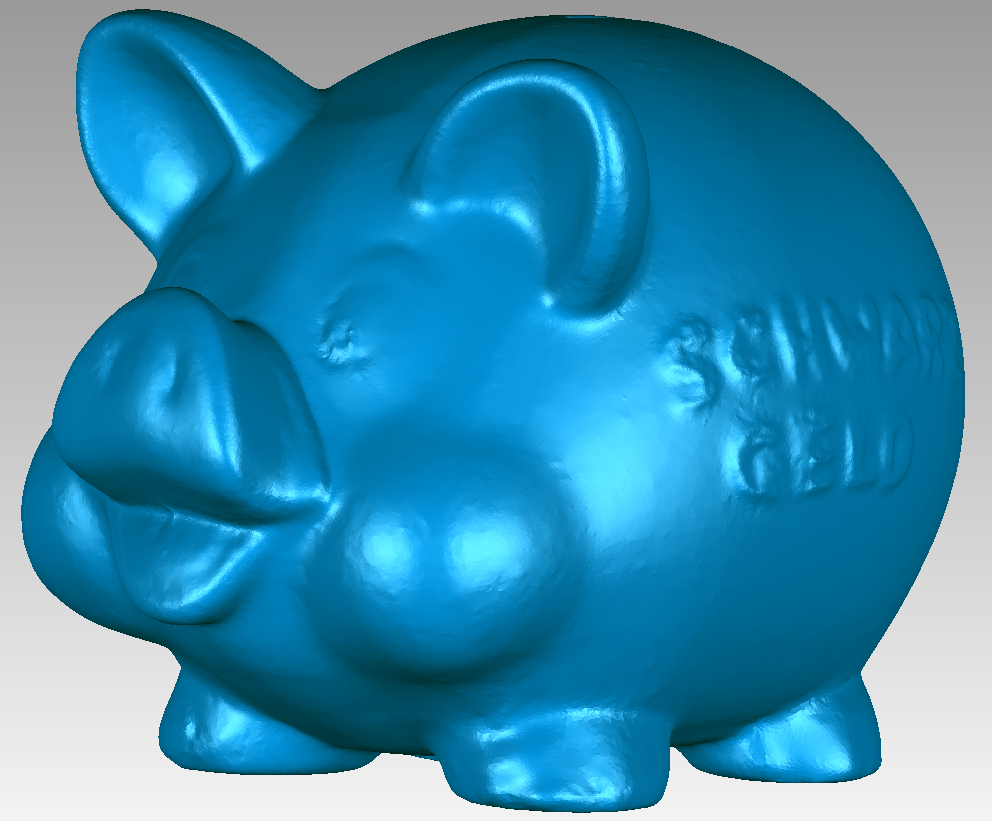
\includegraphics[width=80mm]{images/sparschwein/final} % ersetzen
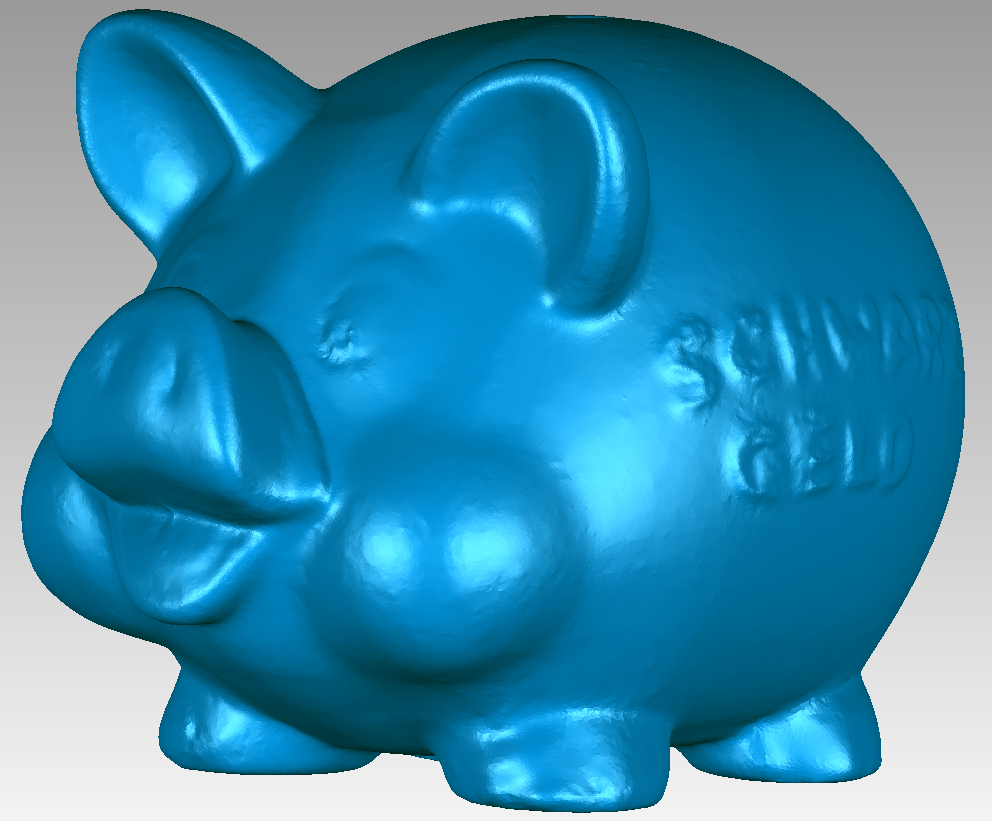
\includegraphics[width=80mm]{images/sparschwein/final}
\end{figure}
		
\end{document}
